\chapter{Testy Systemu}

\section{Przeprowadzane testy}

W celu upewnienia się, że zaimplementowany system działa zgodnie z przeznaczeniem, przeprowadzono testy wydajnościowe, aby ocenić, w jaki sposób system obsługuje liczne żądania wykonywane równolegle, jak i szeregowo. Testy te miały na celu zweryfikowanie zachowania systemu podczas ogólnego użytkowania. Testy zostały wykonane poprzez uruchomienie skryptów powłoki jednocześnie w wielu lokalizacjach.

\section{Platforma testowa}

Testowany system przedstawiony na rys.\ref{testowySystemSchemat} został uruchomiony na jednej fizycznej maszynie podłączonej do sieci lokalnej poprzez kabel ethernet, podczas gdy dodatkowy węzeł protokołu był uruchomiony na Raspberry Pi zero 2W podłączonej do sieci lokalnej poprzez WIFI. Główną testową wartością był czas obsługi żądania.

Parametry platformy testowej to:

\begin{itemize}
    \item Procesor \akronim{CPU} (\english{Central Processing Unit}) - Intel(R) Core(TM) i7-9750H CPU @ 2.60GHz
    \item Dysk twardy - Samsung SSD 980 PRO 1TB
    \item Pamięć \akronim{RAM} (\english{Random-Access Memory}) - Kingston Fury Impact 16GB [1x16GB 2666MHz DDR4 CL15 SODIMM] + Kingston 8 GB DDR4 2666 MHz
\end{itemize}


\begin{figure}[!h]
    \centering
    \includesvg[width=\textwidth]{schemas/tests/testEnvironment.svg}
    \caption{Schemat testowego środowiska}
    \label{testowySystemSchemat}
\end{figure}

\newpage Na rys.\ref{testraspberryPiGraph} przedstawiony został wykres przedstawiający czasy odpowiedzi dla 1000 żądań wykonanych przez Raspberry Pi Zero 2W podłączone przez Wi-Fi do sieci. Wartości wykazują znaczną zmienność, z niektórymi czasami odpowiedzi sięgającymi około 800 milisekund, dłuższy czas przetwarzania pierwszej wiadomości jest spowodowany ustawianiem w systemie wartości niezbędnych do określania ścieżek w sieci \akronim{LAN} (\english{Local Area Network}). Średni czas odpowiedzi wynosi 156,19 milisekund, co jest przedstawione na wykresie czerwoną przerywana linią.

\begin{figure}[!htbp]
    \centering
    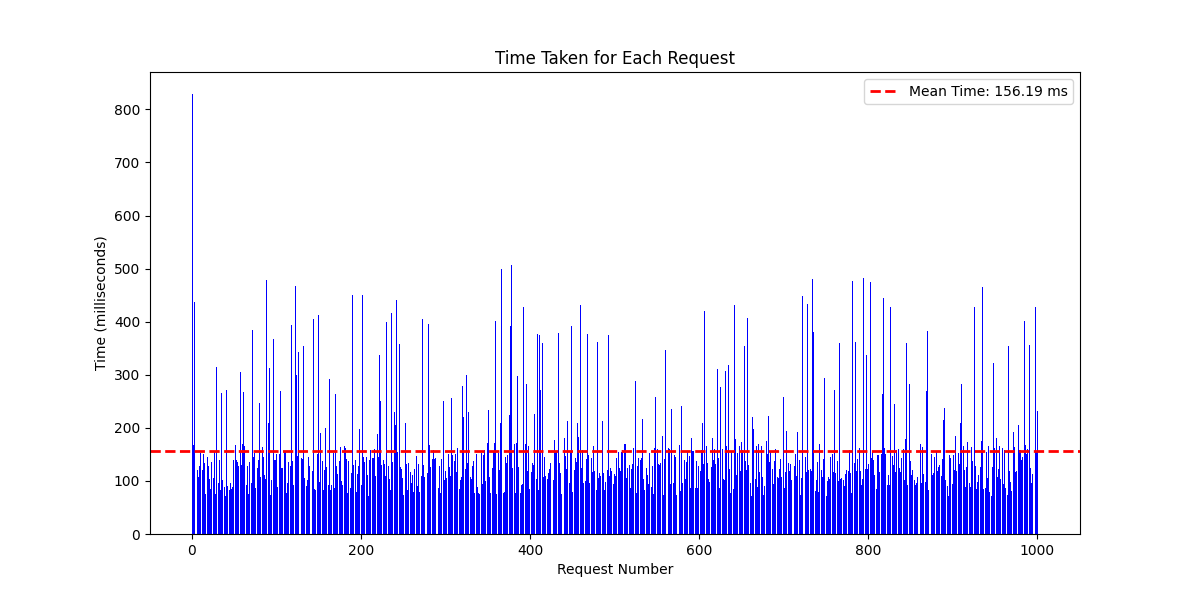
\includegraphics[width=\textwidth]{images/testy/tests.png}
    \caption{Wykres czasu obsługi żądań wysłanych z raspberry pi zero 2W}
    \label{testraspberryPiGraph}
\end{figure}

\newpage Na rys.\ref{testlocalhostGraph} przedstawiony został wykres ilustrujący czasy odpowiedzi dla 1000 żądań wykonanych do platformy testowej (ten sam komputer z uruchomionym systemem). W porównaniu do poprzedniego wykresu, czasy odpowiedzi są zdecydowanie niższe i bardziej spójne, z większością wartości poniżej 100 milisekund. Średni czas odpowiedzi wynosi 64,29 milisekundy, czyli znacznie mniej niż w przypadku uruchomienia testu na Raspberry Pi. Wykres ten pokazuje lepszą wydajność i mniejsze opóźnienia, gdy żądania są wykonywane na tym samym komputerze, omijając opóźnienia związane z siecią.


\begin{figure}[!htbp]
    \centering
    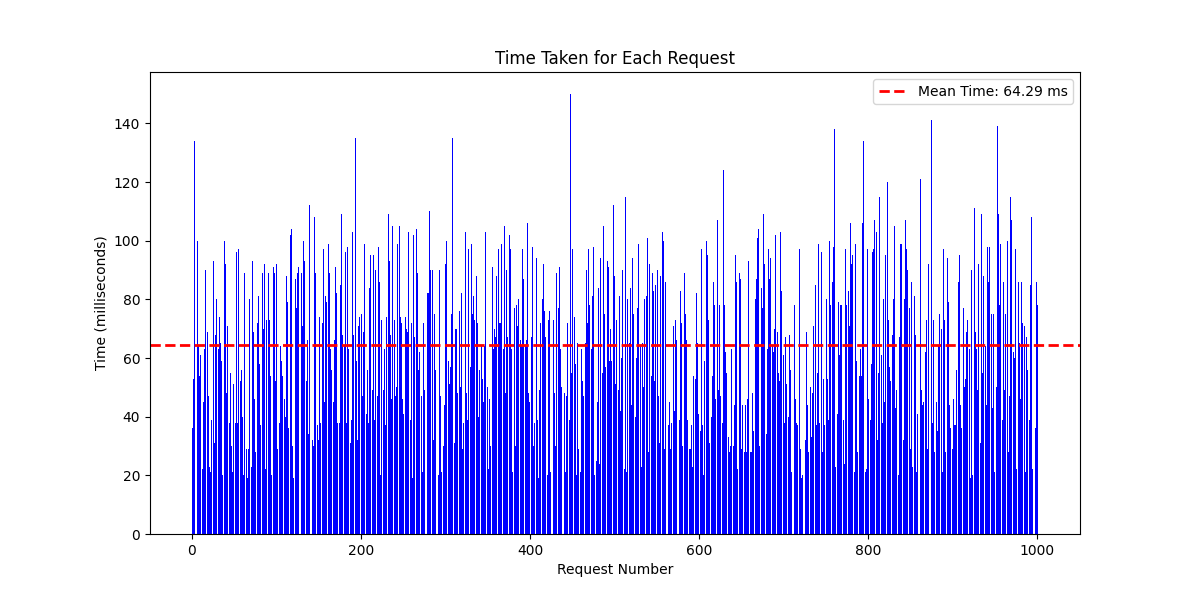
\includegraphics[width=\textwidth]{images/testy/testsLocalhost.png}
    \caption{Wykres czasu obsługi żądań z wysłanych z platformy testowej}
    \label{testlocalhostGraph}
\end{figure}

\newpage Wykonane testy przedstawiają wyraźne porównanie różnic w wydajności w systemie rozproszonym przy wykorzystaniu Wi-Fi oraz aplikacji uruchomionej na tym samym urządzeniu co system, podkreślając wpływ komunikacji sieciowej na czasy odpowiedzi w systemie.
